\section{Child specifications}

\frame{\tableofcontents[currentsection]}


\begin{frame}
    \frametitle{What should a child specification contain?}
    \begin{itemize}
        \item Id for the supervisor
        \item Module, Function \& Arguments (often abbreviated to MFA)
        \item * Restart behaviour (transient, temporary or permanent)
        \item * Type (worker or supervisor)
        \item * Shutdown (timeout or :brutal\_kill)
    \end{itemize}

    \vfill

    \footnotesize
    * values have default values and are thus optional
\end{frame}

\begin{frame}
    \frametitle{How to implement / configure child specs?}
    \begin{itemize}
        \item Through injection
        \item Pass it as a map
        \item Implement the child\_specs(opts) function in the module
    \end{itemize}
\end{frame}

\begin{frame}
    \frametitle{Option 1: through injection}
    \begin{center}
        use GenServer \\
        use Agent \\
        ...
    \end{center}
\end{frame}

\begin{frame}
    \frametitle{Option 1: merits and demerits}
    \begin{columns}

        \begin{column}{0.5\textwidth}
            \begin{itemize}
                \item[+] Easy
                \item[+] Not likely to make mistakes
            \end{itemize}
        \end{column}

        \begin{column}{0.5\textwidth}
            \begin{itemize}
                \item[-] Configuration by default injection
                \item[-] Possible other unwanted injected code
                      \footnotesize
                      \\ e.g. code\_change / doc / default callbacks
            \end{itemize}
        \end{column}
    \end{columns}
\end{frame}

\begin{frame}
    \frametitle{Option 2: pass as a map}
    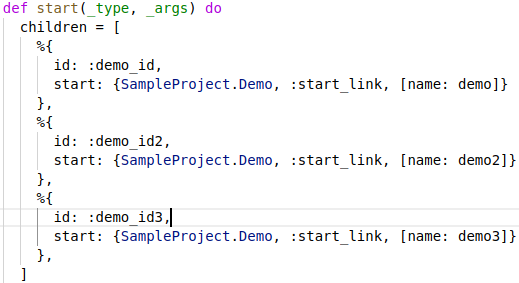
\includegraphics[scale=0.59]{03_pass_children_as_map}
\end{frame}

\begin{frame}
    \frametitle{Option 2: merits and demerits}
    \begin{columns}

        \begin{column}{0.5\textwidth}
            \begin{itemize}
                \item[+] Complete control
                \item[+] No unnecessary extra code
            \end{itemize}
        \end{column}

        \begin{column}{0.5\textwidth}
            \begin{itemize}
                \item[-] Manual ID allocation
                \item[-] Not really open for extension
            \end{itemize}
        \end{column}
    \end{columns}
\end{frame}

\begin{frame}
    \frametitle{Option 3: implement child\_specs/1}
    \code[language=elixir,font=\scriptsize]{demo-code/02_child_spec_caller.ex}
    \code[language=elixir,font=\scriptsize]{demo-code/03_child_spec.ex}
\end{frame}

\begin{frame}
    \frametitle{Option 3: implement child\_specs/1}
    \begin{columns}

        \begin{column}{0.5\textwidth}
            \begin{itemize}
                \item[+] Complete control
                \item[+] Open for extension
                \item[+] Can provide support for dynamic ID's *
            \end{itemize}
        \end{column}

        \begin{column}{0.5\textwidth}
            \begin{itemize}
                \item[-] Needs implementation in your module
                \item[-] More factors have to be considered
                \item[-] A better solution probably already exists
            \end{itemize}
        \end{column}
    \end{columns}
    \vfill
    \footnotesize * Dynamic ID's are not advised with normal supervisors!
\end{frame}